\documentclass[a4paper]{article}
\usepackage{graphicx}

\begin{document}

\begin{figure}
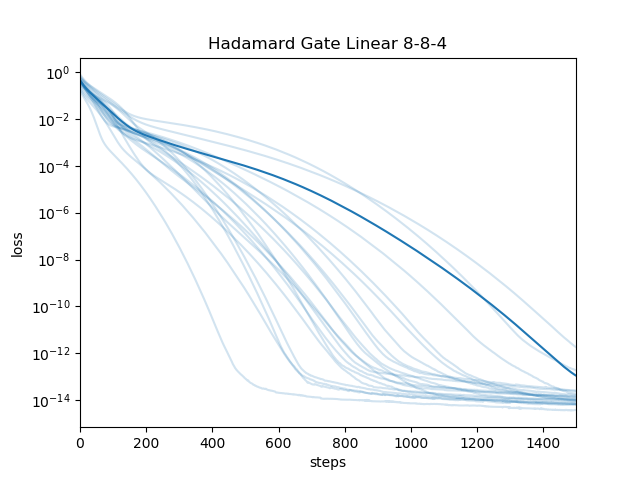
\includegraphics[width=\linewidth]{../figures/8-4-4-traces/sweep_hadamard.png}
\caption{Training a three layer network with 8,8,4 linear activation units on the
hadamard gate. Depicted are 50 training runs with random initialization and different sets
of training samples.}
\label{fig:ltl}
\end{figure}


\begin{figure}
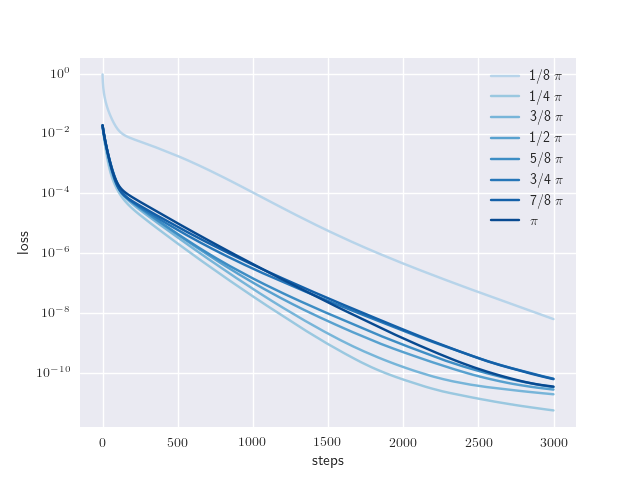
\includegraphics[width=\linewidth]{../figures/rotate_sequential.png}
\caption{Training different rotation gates sequentially on pure states. The same network consisting of 8,8,4 real linear units was trained to fit different rotation gates sequentially on multiples of $1/8 \pi.$ 
After the first training sequence has converged subsequent
training runs begin from a lower starting loss.}
\label{fig:ltl}
\end{figure}

\begin{figure}
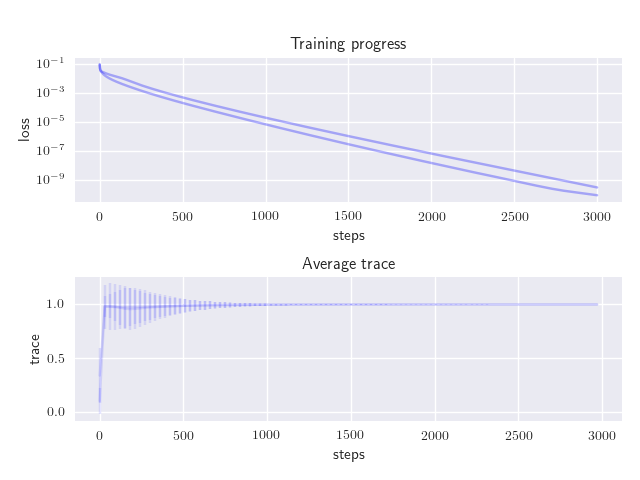
\includegraphics[width=\linewidth]{../figures/density/hadamard/sweep_density_matrix-hadamard_gate.png}
\caption{Training a network to predict density matrices produced by a hadamard gate. Two training
curves are shown in the upper figure and the corresponding mean and standard deviation of the
traces of the predicted density matrices in the lower figure. The traces of the predicted matrices are 
evaluated every 30th training step. The network architecture consists of 16,3,16 linear real units, thereby
forcing the network to make use of the correct number of degrees of freedom.}
\label{fig:density_hadamard}
\end{figure}

\begin{figure}
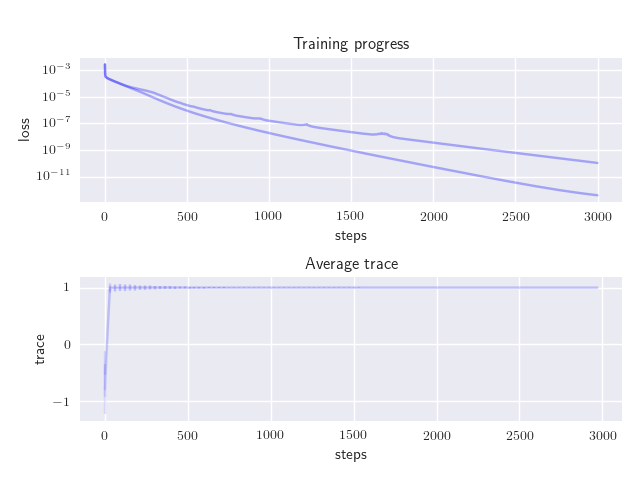
\includegraphics[width=\linewidth]{../figures/density/cnot/sweep_density_matrix-cnot_gate.png}
\caption{Training a network to predict density matrices produced by a CNOT gate. Two training
curves are shown in the upper figure and the corresponding mean and standard deviation of the
traces of the predicted density matrices in the lower figure. The traces of the predicted matrices are
evaluated every 30th training step. The network architecture consistsof 64,16,64 linear real units.}
\label{fig:density_hadamard}
\end{figure}

\begin{figure}
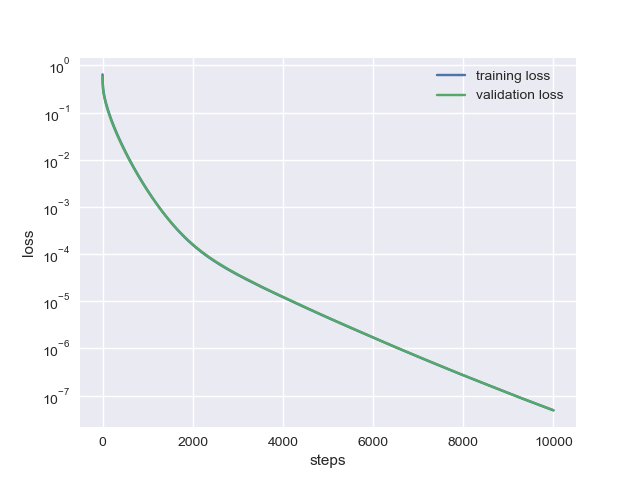
\includegraphics[width=\linewidth]{../figures/relu_4.png}
\caption{Training a one layer relu network on shifted data to prevent dying relus.}
\label{fig:relu_hadamard_4}
\end{figure}

\begin{figure}
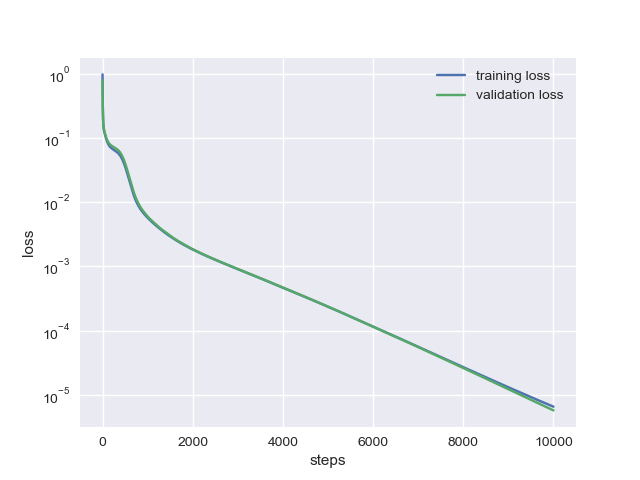
\includegraphics[width=\linewidth]{../figures/relu_8_4.png}
\caption{Training a two layer relu network of 8,4 units on shifted data to prevent dying relus.}
\label{fig:relu_hadamard_8_4}
\end{figure}

\begin{figure}
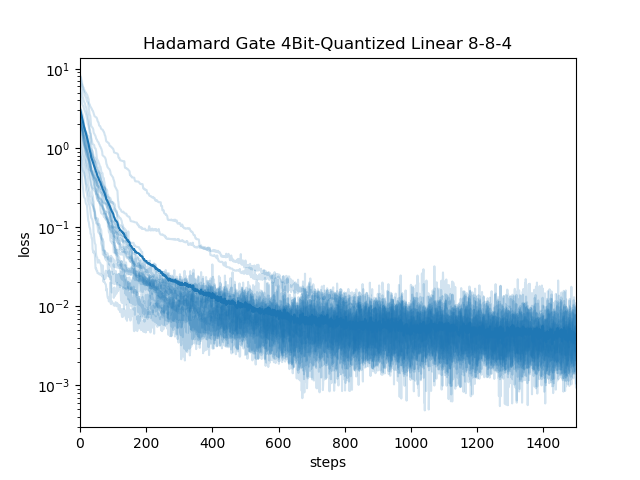
\includegraphics[width=\linewidth]{../figures/8-8-4-traces-quantized/sweep_hadamard-quantized.png}
\caption{Training a three layer network with 4Bit quantized weights and linear activation units. 
The network is fully connected with 8,8,4 units at each layer. Shown are 50 training histories.}
\label{fig:relu_hadamard_8_4}
\end{figure}

\begin{figure}
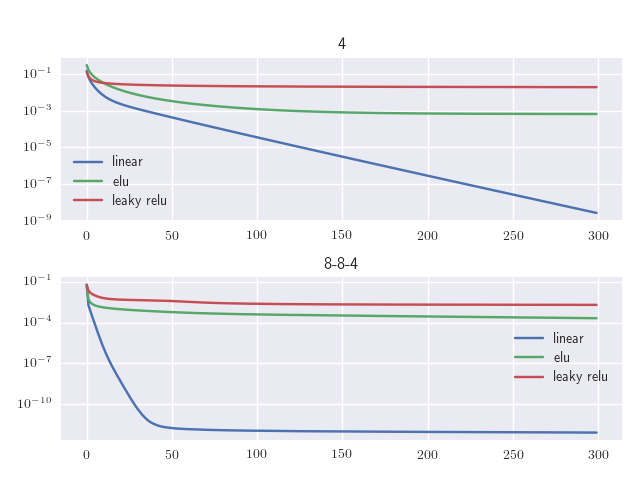
\includegraphics[width=\linewidth]{../figures/non_linear.png}
\caption{Training to predict hadamard gate transformation of 10000 randomly selected pure states.
Depicted in the upper figure are linear regression and worse performing training on
non-linear activation units. Batch size of 32 and adagrad optimizer. The lower figure
depicts training on the same training data set with a 3 three layer network and
different activation units (linear, elu, leaky relu). Again using a batch size of 32 and
adagrad optimizer.
}
\label{fig:relu_hadamard_8_4}
\end{figure}


\end{document}